\chapter{Sorting in Linear Time}

So far, every sorting algorithm you have met -- insertion sort, merge sort,
heapsort, quicksort -- shares one habit. To decide where an element belongs,
the algorithm \emph{compares} it against another element: ``is $a$ less than
$b$?'' It never peeks inside the values; it only asks the universe, over and
over, which of two things is smaller. The very best of these algorithms run in
$\Th(n \log n)$ time, and you might reasonably start to suspect that
$n \log n$ is simply the price of sorting. The cosmic toll. The cost of doing
business.

This chapter is going to do two surprising things. First, it will \emph{prove}
that suspicion partly right: any algorithm that sorts using only comparisons
must, in the worst case, take at least $\Th(n \log n)$ time. That is not a
failure of our cleverness; it is a wall built into the rules of the game. But
second -- and this is the delicious part -- it will show you that the wall has
a door. If you are allowed to look inside the values, to use them as more than
opaque tokens you can only compare, you can sort genuinely faster: in
\emph{linear} time, $\Th(n)$. We will meet three algorithms that walk through
that door: \textbf{counting sort}, \textbf{radix sort}, and
\textbf{bucket sort}.

\begin{focusbox}
The big idea of this chapter, in one breath: \emph{comparisons} are weak. Each
comparison gives you only one bit of information (less, or not less), and you
need a lot of bits to pin down the right ordering, so comparison sorting cannot
beat $\Th(n \log n)$. But if the values themselves carry usable structure --
they are small integers, or fixed-width keys, or uniformly spread reals -- you
can extract information \emph{in bulk} instead of one comparison at a time, and
sorting drops to $\Th(n)$.
\end{focusbox}

\section{Comparisons Are a Kind of Currency}

Let me slow all the way down, because the lower bound is the conceptual heart
of the chapter and it is easy to nod along without really seeing it.

Suppose I hand you three numbers in three sealed boxes, labelled $A$, $B$, $C$.
You cannot see the numbers. Your only allowed move is to point at two boxes and
ask me ``is the number in this one smaller than the number in that one?'' I
answer yes or no, truthfully. Your job is to tell me the correct sorted order
of the three boxes.

How many questions might you need? Let us count the possible answers you might
have to produce. With three distinct values, the sorted order could be any of
the $3! = 6$ permutations:
\[
ABC,\quad ACB,\quad BAC,\quad BCA,\quad CAB,\quad CBA.
\]
Each of these is a genuinely different answer, and before you ask anything you
have no idea which one is correct. Every question you ask gets a yes/no answer,
which at best splits the still-possible answers into two groups. The best you
can hope for from one question is to cut the number of surviving possibilities
in half.

\begin{intuitionbox}
Think of it as a guessing game. There are $6$ secret answers on the table. Each
yes/no question can, at most, cut the pile in half. After one question: at
least $3$ left. After two: at least $\ceil{3/2} = 2$ left. After three: at
least $1$. You cannot guarantee you have narrowed it to a single answer in
fewer than $\ceil{\log_2 6} = 3$ questions, because two questions can only
distinguish $2^2 = 4$ outcomes, and $4 < 6$. There simply are not enough
yes/no patterns to go around.
\end{intuitionbox}

That is the entire argument, and it scales. To sort $n$ elements you must be
able to produce any of $n!$ possible orderings. Each comparison is one yes/no
question. A sequence of $k$ comparisons produces a pattern of $k$ bits, and
there are only $2^k$ distinct bit-patterns. If your algorithm always finishes
in $k$ comparisons, then those $2^k$ patterns must cover all $n!$ answers --
otherwise two different correct orderings would produce the same pattern of
answers, and the algorithm could not tell them apart. So we need
$2^k \ge n!$, which forces $k \ge \log_2(n!)$.

\subsection{The Decision Tree: Drawing the Argument}

The clean way to make this rigorous is to draw the algorithm as a tree, called
a \emph{decision tree}. Forget the algorithm's code for a moment and watch only
its comparisons. The first comparison it makes is the root. Depending on the
yes/no answer, it goes left or right to its next comparison, and so on. Every
internal node is a comparison; every leaf is a final answer (a permutation).

\begin{figure}[H]
\centering
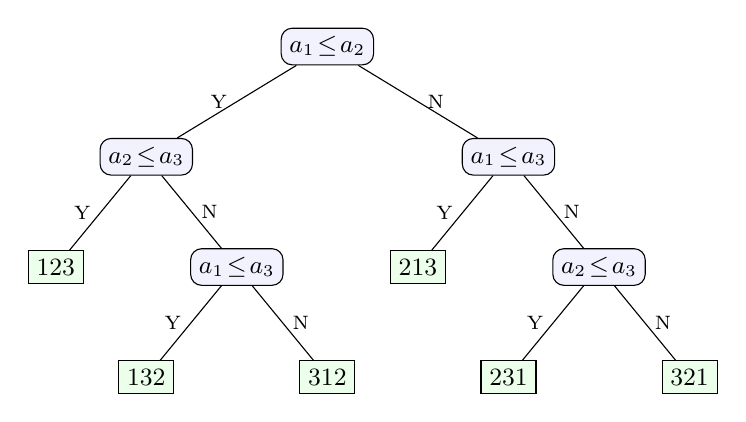
\begin{tikzpicture}[
  every node/.style={font=\small},
  cmp/.style={draw, rounded corners, fill=blue!5, inner sep=3pt},
  leaf/.style={draw, fill=green!8, inner sep=3pt},
  level distance=14mm,
  level 1/.style={sibling distance=46mm},
  level 2/.style={sibling distance=23mm},
]
\node[cmp]{$a_1 \!\le\! a_2$}
  child {node[cmp]{$a_2 \!\le\! a_3$}
    child {node[leaf]{$123$} edge from parent node[left,font=\scriptsize]{Y}}
    child {node[cmp]{$a_1 \!\le\! a_3$}
      child {node[leaf]{$132$} edge from parent node[left,font=\scriptsize]{Y}}
      child {node[leaf]{$312$} edge from parent node[right,font=\scriptsize]{N}}
      edge from parent node[right,font=\scriptsize]{N}}
    edge from parent node[left,font=\scriptsize]{Y}}
  child {node[cmp]{$a_1 \!\le\! a_3$}
    child {node[leaf]{$213$} edge from parent node[left,font=\scriptsize]{Y}}
    child {node[cmp]{$a_2 \!\le\! a_3$}
      child {node[leaf]{$231$} edge from parent node[left,font=\scriptsize]{Y}}
      child {node[leaf]{$321$} edge from parent node[right,font=\scriptsize]{N}}
      edge from parent node[right,font=\scriptsize]{N}}
    edge from parent node[right,font=\scriptsize]{N}};
\end{tikzpicture}
\caption{A decision tree for sorting three elements. Each internal node is a
comparison; ``Y''/``N'' edges record the answer. A leaf labelled $ijk$ means
the sorted order is $a_i \le a_j \le a_k$. There are $3! = 6$ leaves, one per
permutation, and the deepest leaf is $3$ comparisons down.}
\label{ch08:decision-tree}
\end{figure}

In Figure~\ref{ch08:decision-tree}, \emph{running} the algorithm
on a particular input means starting at the root and walking down to a leaf,
turning left or right according to each comparison's answer. The number of
comparisons that run makes on that input is exactly the length of the path it
walks -- the \emph{depth} of the leaf it reaches. The \emph{worst-case} number
of comparisons is the depth of the deepest leaf: the \emph{height} of the tree.

So the question ``how few comparisons can a sorting algorithm guarantee?''
becomes a question about trees: how \emph{short} can a tree be if it must have
at least $n!$ leaves?

\begin{formalbox}
\textbf{Two facts about binary trees we will lean on.}
A binary tree of height $h$ has at most $2^h$ leaves -- because each level
doubles the count of nodes available, and the leaves all live at depth $\le h$.
Turned around: a binary tree with $L$ leaves has height at least $\log_2 L$.
\end{formalbox}

\subsection{The Lower Bound, Stated and Proved}

\begin{theorem}[Comparison-sort lower bound]
\label{ch08:lower-bound}
Any comparison sort, in the worst case, performs $\Om(n \log n)$ comparisons to
sort $n$ elements. Concretely, its decision tree has height at least
$\log_2(n!) = \Th(n \log n)$.
\end{theorem}

\begin{proof}
Consider any comparison sort and its decision tree $T$ on inputs of length $n$.
Because the algorithm must be \emph{correct}, every one of the $n!$ possible
orderings of the input must appear as the label of at least one reachable leaf;
if some permutation $\pi$ labelled no leaf, then the input whose correct answer
is $\pi$ would be sorted wrongly. Hence $T$ has at least $n!$ leaves.

A binary tree with at least $n!$ leaves has height
$h \ge \log_2(n!)$. The worst-case comparison count is exactly $h$, so the
algorithm makes at least $\log_2(n!)$ comparisons on some input.

It remains to see that $\log_2(n!) = \Th(n\log n)$. The upper side is easy:
$n! \le n^n$, so $\log_2(n!) \le n \log_2 n$. For the lower side, keep only the
top half of the factors,
\[
n! \;=\; n\cdot(n-1)\cdots 2 \cdot 1 \;\ge\; \underbrace{n\cdot(n-1)\cdots
\tfrac{n}{2}}_{n/2 \text{ factors, each } \ge\, n/2}\;\ge\;
\Bigl(\frac{n}{2}\Bigr)^{n/2},
\]
so $\log_2(n!) \ge \frac{n}{2}\log_2\frac{n}{2} = \frac{n}{2}(\log_2 n - 1) =
\Om(n\log n)$. Both bounds together give $\log_2(n!) = \Th(n \log n)$.
\end{proof}

\begin{corollary}
Merge sort and heapsort are asymptotically optimal comparison sorts: their
$\Oh(n\log n)$ worst-case running time matches the $\Om(n\log n)$ lower bound
to within a constant factor.
\end{corollary}

\begin{trapbox}
The lower bound is about \emph{comparison} sorts, and only about them. It says
nothing about algorithms that do other things with the keys -- adding them up,
indexing an array with them, slicing them into digits. People sometimes
over-read Theorem~\ref{ch08:lower-bound} as ``sorting is $\Om(n\log n)$,
period.'' It is not. It is ``\emph{comparison-based} sorting is
$\Om(n\log n)$.'' The rest of this chapter is a tour of what becomes possible
the moment you stop limiting yourself to comparisons.
\end{trapbox}

\begin{walkbox}
Here is something to chew on while you walk. The proof only needs the tree to
have $\ge n!$ leaves and to be \emph{binary}. Where exactly did ``binary'' come
from? It came from each comparison having two outcomes. Now imagine a magical
machine whose every probe has \emph{three} outcomes (less, equal, greater).
Redo the counting. Does three-way branching break the $\Om(n\log n)$ barrier,
or does it only change the base of the logarithm -- and why does changing the
base of a logarithm not change a $\Th(n\log n)$ bound at all?
\end{walkbox}

\begin{historybox}
This is CLRS Chapter~8, ``Sorting in Linear Time.'' The decision-tree lower
bound is Section~8.1; counting sort is~8.2; radix sort is~8.3; bucket sort
is~8.4. The information-theoretic flavour of the argument -- ``you need
$\log_2(n!)$ bits, and each comparison yields one bit'' -- is the same idea that
underlies Shannon's information theory and shows up again whenever someone
proves that a problem \emph{cannot} be solved faster than some bound. Lower
bounds like this are rarer and, in a sense, deeper than algorithms: an
algorithm shows one way is possible, but a lower bound rules out \emph{all}
ways at once.
\end{historybox}

\section{Counting Sort: Sorting Without Comparing}

Now for the first door through the wall. Counting sort sorts integers without
ever comparing two of them. Instead it asks a different question about each
element: ``\emph{what} are you?'' -- and uses the answer as an array index.

\begin{intuitionbox}
Picture a classroom of students, each holding a card with a single digit
$0$--$9$. You want them lined up in sorted order. Instead of comparing cards
pairwise, you put ten labelled bins on the floor -- bin $0$ through bin $9$ --
and shout ``put your card in the bin that matches your digit.'' Now just sweep
the bins left to right and read the cards out. They come out sorted, and you
never compared a single pair. The cost was one pass to fill bins and one pass
to drain them: linear. That is counting sort. The catch, already visible, is
that you needed one bin per possible value, so this only works when the values
come from a small, known range.
\end{intuitionbox}

\subsection{The Setup}

Counting sort assumes the $n$ input values are integers in a known range
$\{0, 1, \dots, k\}$. The plan:

\begin{enumerate}
\item \textbf{Count.} Make an array $C[0\,..\,k]$ and set $C[v]$ to the number
of input elements equal to $v$. (One pass over the input.)
\item \textbf{Accumulate.} Turn $C$ into a running total, so that $C[v]$ becomes
the number of elements \emph{less than or equal to} $v$. Now $C[v]$ tells you
the last position in the sorted output where a value $v$ belongs.
\item \textbf{Place.} Walk the input and drop each element into its computed
output slot, decrementing $C[v]$ as you go so equal elements stack up neatly.
\end{enumerate}

\begin{algorithm}[H]
\caption{\textsc{Counting-Sort}}
\KwIn{Array $A[1\,..\,n]$ of integers, each in $\{0,\dots,k\}$.}
\KwOut{Array $B[1\,..\,n]$ holding the elements of $A$ in sorted order.}
let $C[0\,..\,k]$ be a new array\;
\For{$v \leftarrow 0$ \KwTo $k$}{$C[v] \leftarrow 0$\;}
\For{$j \leftarrow 1$ \KwTo $n$}{$C[A[j]] \leftarrow C[A[j]] + 1$\tcp*{$C[v]$ now counts how many equal $v$}}
\For{$v \leftarrow 1$ \KwTo $k$}{$C[v] \leftarrow C[v] + C[v-1]$\tcp*{$C[v]$ now counts how many $\le v$}}
\For{$j \leftarrow n$ \KwTo $1$}{
  $B[\,C[A[j]]\,] \leftarrow A[j]$\;
  $C[A[j]] \leftarrow C[A[j]] - 1$\;
}
\Return $B$\;
\end{algorithm}

The single subtle choice is the \emph{last} loop running \emph{backwards},
from $n$ down to $1$. Hold that thought; it is what makes counting sort
\emph{stable}, and stability is exactly what radix sort will demand of it in
the next section.

\subsection{A Full Numeric Trace}

Let us sort
\[
A = (2,\; 5,\; 3,\; 0,\; 2,\; 3,\; 0,\; 3),\qquad n = 8,\quad k = 5.
\]

\textbf{Step 1 -- count.} Sweep $A$ and tally each value:
\[
\begin{array}{c|cccccc}
v      & 0 & 1 & 2 & 3 & 4 & 5\\\hline
C[v]   & 2 & 0 & 2 & 3 & 0 & 1
\end{array}
\]
(Two $0$s, no $1$s, two $2$s, three $3$s, no $4$s, one $5$. They sum to $8$,
good.)

\textbf{Step 2 -- accumulate} into running totals ``how many $\le v$'':
\[
\begin{array}{c|cccccc}
v      & 0 & 1 & 2 & 3 & 4 & 5\\\hline
C[v]   & 2 & 2 & 4 & 7 & 7 & 8
\end{array}
\]
Read $C[3] = 7$ as ``there are $7$ elements $\le 3$, so the last $3$ belongs in
slot $7$ of the output.''

\textbf{Step 3 -- place}, scanning $A$ from right ($j=8$) to left ($j=1$). At
each step we read $A[j]$, look up $C[A[j]]$ to get the slot, write into $B$, and
decrement.

\begin{center}
\begin{tabular}{c|c|c|c|l}
$j$ & $A[j]$ & slot $C[A[j]]$ & write & then $C$ becomes\\\hline
$8$ & $3$ & $7$ & $B[7]=3$ & $C[3]\!:7\!\to\!6$\\
$7$ & $0$ & $2$ & $B[2]=0$ & $C[0]\!:2\!\to\!1$\\
$6$ & $3$ & $6$ & $B[6]=3$ & $C[3]\!:6\!\to\!5$\\
$5$ & $2$ & $4$ & $B[4]=2$ & $C[2]\!:4\!\to\!3$\\
$4$ & $0$ & $1$ & $B[1]=0$ & $C[0]\!:1\!\to\!0$\\
$3$ & $3$ & $5$ & $B[5]=3$ & $C[3]\!:5\!\to\!4$\\
$2$ & $5$ & $8$ & $B[8]=5$ & $C[5]\!:8\!\to\!7$\\
$1$ & $2$ & $3$ & $B[3]=2$ & $C[2]\!:3\!\to\!2$\\
\end{tabular}
\end{center}

Collecting the writes by slot index gives
\[
B = (\,0,\;0,\;2,\;2,\;3,\;3,\;3,\;5\,),
\]
which is exactly $A$ in sorted order. Notice we never asked ``is this bigger
than that?'' even once.

Figure~\ref{ch08:counting-place} shows what the placement step is really doing:
the accumulated array $C$ hands each value a \emph{block} of output slots, and
the contiguity of those blocks is what makes the writes land in sorted order
with no comparisons.

\begin{figure}[H]
\centering
\begin{tikzpicture}[font=\small,
  cell/.style={draw, minimum width=7mm, minimum height=7mm},
  lab/.style={font=\scriptsize, gray}]
  % output array B, slots 1..8
  \foreach \i/\val in {1/0,2/0,3/2,4/2,5/3,6/3,7/3,8/5} {
    \node[cell] (s\i) at (\i*0.8,0) {\val};
    \node[lab, below=0pt of s\i] {\i};
  }
  \node[left=2mm of s1] {$B:$};
  % brace groups for each value's block
  \draw[decorate, decoration={brace, amplitude=4pt}, sourceblue]
    ($(s1.north west)+(0,1mm)$) -- ($(s2.north east)+(0,1mm)$)
    node[midway, above=3pt, sourceblue]{value $0$ (slots $1$--$2$)};
  \draw[decorate, decoration={brace, amplitude=4pt}, targetgreen]
    ($(s3.north west)+(0,1mm)$) -- ($(s4.north east)+(0,1mm)$)
    node[midway, above=3pt, targetgreen]{$2$ ($3$--$4$)};
  \draw[decorate, decoration={brace, amplitude=4pt}, quotientorange]
    ($(s5.north west)+(0,1mm)$) -- ($(s7.north east)+(0,1mm)$)
    node[midway, above=3pt, quotientorange]{$3$ ($5$--$7$)};
  \draw[decorate, decoration={brace, amplitude=4pt}, structurepurple]
    ($(s8.north west)+(0,1mm)$) -- ($(s8.north east)+(0,1mm)$)
    node[midway, above=3pt, structurepurple]{$5$ ($8$)};
\end{tikzpicture}
\caption{After accumulation, $C$ reserves a contiguous block of output slots for
each value: value $v$ owns slots $C[v-1]+1$ through $C[v]$. The placement loop
fills each block from its high end downward, which is why scanning the input
right-to-left makes the sort stable.}
\label{ch08:counting-place}
\end{figure}

\begin{labbox}
Trace it yourself, but flip the final loop to run \emph{forwards}, $j$ from $1$
to $n$, with everything else unchanged. You will find it still sorts! So why do
we insist on going backwards? Re-run both directions on an input where you can
\emph{tell the equal elements apart} -- say, tag them: $3_a, 3_b, 3_c$ in their
original left-to-right order. With the backward loop, do $3_a, 3_b, 3_c$ come
out in their original relative order in $B$? With the forward loop, what happens
to that order? The answer is the whole point of the next box.
\end{labbox}

\subsection{Stability, and Why We Care}

\begin{definition}[Stable sort]
A sort is \emph{stable} if elements that compare equal keep their original
relative order in the output. If $3_a$ appeared before $3_b$ in the input, a
stable sort guarantees $3_a$ still appears before $3_b$ in the output.
\end{definition}

Counting sort as written is stable. Here is the gentle reason. The accumulated
$C[v]$ marks the \emph{last} output slot for value $v$, and we fill from the
back. So the \emph{rightmost} input element of value $v$ grabs the highest slot,
and as we move leftward through the input, each earlier element of value $v$
grabs the next-lower slot. Earlier-in-input lands earlier-in-output: that is
exactly stability. Run the loop forward instead and the order of equal elements
reverses -- still sorted, but no longer stable.

\begin{focusbox}
Two properties of counting sort to carry forward: it is \textbf{linear} in
$n + k$, and it is \textbf{stable}. Radix sort, coming next, leans on
\emph{both} -- it would simply not work without stability.
\end{focusbox}

\subsection{Cost, and the Catch}

\begin{complexitybox}
\textbf{Counting sort.}
\begin{itemize}
\item Initialize $C$: $\Th(k)$.
\item Count: $\Th(n)$.
\item Accumulate: $\Th(k)$.
\item Place: $\Th(n)$.
\end{itemize}
Total time $\Th(n + k)$. Extra space $\Th(n + k)$ (the output $B$ and the
counter $C$). When $k = \Oh(n)$ -- the range is no bigger than the count of
elements -- this is $\Th(n)$: \emph{linear} sorting, beating the $n\log n$
wall.
\end{complexitybox}

\begin{trapbox}
The catch lives in that innocent ``$+\,k$''. If your values are $32$-bit
integers, then $k$ could be about $4{,}000{,}000{,}000$, and counting sort would
allocate a four-billion-entry array to sort, say, ten numbers. That is a
catastrophe of both time and memory. Counting sort is only a good idea when the
range $k$ is comparable to (or smaller than) the number of elements $n$. The
moment $k \gg n$, you want a different tool -- which is precisely the gap radix
sort fills.
\end{trapbox}

\section{Radix Sort: Many Small Sorts Make One Big Sort}

Counting sort is wonderful but only for a small range. What if your keys are big
-- $32$-bit integers, or words, or dates? The trick of \emph{radix sort} is to
chop each key into small \emph{digits} and sort by one digit at a time, using a
stable sort (counting sort!) for each pass. The digit's range is small, so each
pass is cheap; and by ordering the passes cleverly, the small sorts compose into
a full sort.

\subsection{Least Significant Digit First -- and Why That Order}

The counterintuitive rule is: sort by the \emph{least} significant digit first,
then the next, and finish with the \emph{most} significant digit.

\begin{intuitionbox}
Sorting most-significant-digit-first feels natural -- it is how you would
alphabetize by hand -- but it forces you to recurse into ever-smaller groups and
keep them separated. Least-significant-first is the magic trick: because each
pass is \emph{stable}, sorting on a higher digit never disturbs the relative
order already established by the lower digits. Each pass refines the previous
one. After the last (most significant) pass, ties on the top digit are broken by
the order from the previous pass, whose ties are broken by the pass before, all
the way down. The whole number ends up sorted.
\end{intuitionbox}

\begin{algorithm}[H]
\caption{\textsc{Radix-Sort}}
\KwIn{Array $A[1\,..\,n]$ of $d$-digit numbers; digit $1$ is least significant.}
\KwOut{$A$ sorted into nondecreasing order.}
\For{$i \leftarrow 1$ \KwTo $d$}{
  use a \emph{stable} sort to sort array $A$ on digit $i$\;
}
\Return $A$\;
\end{algorithm}

\subsection{A Full Numeric Trace}

Sort these seven three-digit numbers:
\[
329,\; 457,\; 657,\; 839,\; 436,\; 720,\; 355.
\]
That is $n = 7$; I will line them up in columns and sort digit by digit, using
a stable sort on each column. The base is $10$, so each digit ranges over
$0$--$9$.

\[
\begin{array}{c@{\qquad}c@{\qquad}c@{\qquad}c}
\textbf{input} & \textbf{by 1's} & \textbf{by 10's} & \textbf{by 100's}\\[2pt]
329 & 72\underline{0} & 7\underline{2}0 & \underline{3}29\\
457 & 35\underline{5} & 3\underline{2}9 & \underline{3}55\\
657 & 43\underline{6} & 4\underline{3}6 & \underline{4}36\\
839 & 45\underline{7} & 8\underline{3}9 & \underline{4}57\\
436 & 65\underline{7} & 3\underline{5}5 & \underline{6}57\\
720 & 32\underline{9} & 4\underline{5}7 & \underline{7}20\\
355 & 83\underline{9} & 6\underline{5}7 & \underline{8}39\\
\end{array}
\]

Read it left to right. Column~2 sorts by the units digit only (underlined);
note $457$ and $657$ both end in $7$ and, because the sort is stable, $457$
stays ahead of $657$ exactly as it was in the units-sorted column. Column~3
sorts that result by the tens digit; again ties (like $355$ vs.\ $457$, both
tens digit $5$) keep the order the units pass gave them. Column~4 sorts by the
hundreds digit, and we are done:
\[
329,\; 355,\; 436,\; 457,\; 657,\; 720,\; 839.
\]
Sorted. Let me show the stability paying off precisely. After the tens pass, the
order among the $5$-tens group is $355, 457, 657$ -- and that came purely from
their units digits: $355$ leads because its units digit $5$ is smallest, while
$457$ and $657$ tie on units digit $7$ and so keep the order the units pass
already gave them. When the hundreds pass scatters them, that internal order
survives wherever the hundreds digits agree.

Figure~\ref{ch08:radix-stable} isolates that single moment: the tens pass moves
$355$, $457$, and $657$ around, but because they share the same tens digit, the
order the units pass established travels with them untouched.

\begin{figure}[H]
\centering
\begin{tikzpicture}[font=\small,
  box/.style={draw, minimum width=10mm, minimum height=7mm, rounded corners},
  hl/.style={draw, fill=quotientorange!18, minimum width=10mm, minimum height=7mm, rounded corners}]
  % before: after units pass
  \foreach \i/\val/\st in {1/720/box,2/355/hl,3/436/box,4/457/hl,5/657/hl,6/329/box,7/839/box} {
    \node[\st] (a\i) at (\i*1.15,0) {\val};
  }
  \node[left=2mm of a1] {after units pass:};
  % after: after tens pass
  \foreach \i/\val/\st in {1/720/box,2/329/box,3/436/box,4/839/box,5/355/hl,6/457/hl,7/657/hl} {
    \node[\st] (b\i) at (\i*1.15,-2.0) {\val};
  }
  \node[left=2mm of b1] {after tens pass:};
  % arrows tracing the three highlighted elements
  \draw[->, quotientorange, thick] (a2.south) to[bend right=10] (b5.north);
  \draw[->, quotientorange, thick] (a4.south) to[bend right=8] (b6.north);
  \draw[->, quotientorange, thick] (a5.south) to[bend right=6] (b7.north);
\end{tikzpicture}
\caption{Stability in action during the tens pass. The three shaded elements
($355, 457, 657$) all have tens digit $5$, so the tens pass must keep their
relative order; the arrows show that the order $355, 457, 657$ -- earned by the
earlier units pass -- is carried over intact. A non-stable sort would be free to
permute them and break the result.}
\label{ch08:radix-stable}
\end{figure}

\begin{focusbox}
The invariant that makes radix sort correct: \emph{after the pass on digit $i$,
the array is sorted according to the low-order $i$ digits treated as a single
number.} The base case ($i = 0$) is trivially true. Each stable pass on digit
$i+1$ preserves it. After $d$ passes, the array is sorted on all $d$ digits --
i.e., fully sorted.
\end{focusbox}

\begin{formalbox}
\textbf{Why the inductive step holds.} Assume after pass $i$ the array is sorted
on the low $i$ digits. Now stably sort on digit $i+1$. Take any two elements
$x, y$.
\emph{(a)} If they differ on digit $i+1$, the new pass orders them correctly by
that digit, which dominates all lower digits -- correct.
\emph{(b)} If they agree on digit $i+1$, stability keeps their pre-pass relative
order, which by the inductive hypothesis already reflects the low $i$ digits --
correct. Either way the array is now sorted on the low $i+1$ digits.
\end{formalbox}

\begin{trapbox}
Radix sort is correct \emph{only because each pass is stable}. Swap in an
unstable per-digit sort and it breaks: a later pass on a higher digit would
scramble the careful ordering the lower digits had earned. This is the deep
reason we built counting sort to be stable. If you find yourself ``optimizing''
radix sort by dropping in quicksort per digit, you have quietly broken it.
\end{trapbox}

\subsection{Cost}

Each of the $d$ passes is a counting sort over a digit, whose range is the base
$b$ (for decimal digits, $b = 10$). One pass costs $\Th(n + b)$, and there are
$d$ passes:
\[
T(n) = \Th\bigl(d\,(n + b)\bigr).
\]

There is a lovely tuning knob here. Suppose the keys are $w$ bits wide. You may
slice them into digits of any width $r$ bits you like; then each digit ranges
over $b = 2^r$ values and there are $d = \ceil{w/r}$ digits. Substituting:
\[
T(n) = \Th\!\left(\frac{w}{r}\,(n + 2^r)\right).
\]
Choosing $r = \log_2 n$ (so $2^r = n$) makes each pass cost $\Th(n)$ and gives
\[
T(n) = \Th\!\left(\frac{w}{\log_2 n}\,n\right).
\]
If the word width $w$ is a constant number of machine words -- as it is for
ordinary $32$- or $64$-bit integers -- then $w = \Oh(\log n)$ on inputs large
enough to address, and this collapses to $\Th(n)$. \emph{Linear} again.

\begin{complexitybox}
\textbf{Radix sort} on $n$ keys of $d$ digits in base $b$: time
$\Th\bigl(d(n+b)\bigr)$, stable, extra space $\Th(n + b)$. With digit width
tuned to $r=\log_2 n$ for $w$-bit keys: $\Th\!\bigl(\tfrac{w}{\log n}\,n\bigr)$,
which is $\Th(n)$ whenever $w = \Oh(\log n)$.
\end{complexitybox}

\begin{aestheticbox}
Radix sort is not a museum piece. It is how you sort huge files of fixed-width
keys fast: sorting billions of $64$-bit integers, network packets by IP address,
strings of bounded length, database columns. GPU and large-scale sorting
routines very often \emph{are} radix sorts, because each pass is a simple,
cache-friendly, embarrassingly parallel counting pass with no branchy
comparisons. When people say ``we sorted a terabyte in record time,'' a radix
sort is frequently doing the heavy lifting underneath.
\end{aestheticbox}

\begin{walkbox}
A puzzle for the walk. Radix sort's cost has that $d$ factor, and merge sort is
$\Th(n \log n)$, so which one wins comes down to $d$ versus $\log n$. When
you sort $n$ distinct integers, how many bits $w$ do you \emph{at minimum} need
just to give them distinct values? What does that say about $d$ relative to
$\log n$, and does radix sort's apparent ``linear'' speed quietly smuggle a
$\log n$ back in through the word width? (There is a real and much-argued
subtlety here. Sit with it.)
\end{walkbox}

\section{Bucket Sort: Betting on the Distribution}

The last linear-time sorter changes the assumption entirely. Counting and radix
sort require integer (or integer-like) keys. Bucket sort instead assumes the
inputs are \emph{real numbers drawn uniformly at random} from an interval, say
$[0, 1)$. Under that assumption it runs in linear time \emph{on average}.

\begin{intuitionbox}
If $n$ numbers are sprinkled uniformly over $[0,1)$, then chopping the interval
into $n$ equal slots -- $[0, \tfrac1n), [\tfrac1n, \tfrac2n), \dots$ -- should
catch roughly one number per slot. So: scatter every number into its slot
(cheap, just multiply by $n$ and take the floor), sort each tiny slot with any
simple method (they are nearly empty, so this is cheap), then read the slots out
in order. Because uniform inputs spread evenly, no slot gets crowded, and the
total work stays linear. You are \emph{betting} on the distribution; when the
bet is right, you win big.
\end{intuitionbox}

\begin{algorithm}[H]
\caption{\textsc{Bucket-Sort}}
\KwIn{Array $A[1\,..\,n]$ with each $A[j] \in [0,1)$.}
\KwOut{The elements of $A$ in sorted order.}
let $\mathit{Bk}[0\,..\,n-1]$ be an array of empty lists\;
\For{$j \leftarrow 1$ \KwTo $n$}{
  insert $A[j]$ into list $\mathit{Bk}[\,\floor{n \cdot A[j]}\,]$\;
}
\For{$i \leftarrow 0$ \KwTo $n-1$}{
  sort list $\mathit{Bk}[i]$ with insertion sort\;
}
\Return the lists $\mathit{Bk}[0], \mathit{Bk}[1], \dots,
\mathit{Bk}[n-1]$ concatenated in order\;
\end{algorithm}

\subsection{A Numeric Trace}

Take $n = 10$ and the inputs
\[
.78,\;.17,\;.39,\;.26,\;.72,\;.94,\;.21,\;.12,\;.23,\;.68.
\]
With $n = 10$, the bucket index of value $x$ is $\floor{10x}$ -- just the first
decimal digit. Scatter:

\begin{center}
\begin{tabular}{c|l}
bucket & contents (in arrival order)\\\hline
$0$ & --\\
$1$ & $.17,\; .12$\\
$2$ & $.26,\; .21,\; .23$\\
$3$ & $.39$\\
$4$ & --\\
$5$ & --\\
$6$ & $.68$\\
$7$ & $.78,\; .72$\\
$8$ & --\\
$9$ & $.94$\\
\end{tabular}
\end{center}

Now insertion-sort each bucket (most have $0$ or $1$ element, so there is
nothing to do; bucket $1$ becomes $.12, .17$; bucket $2$ becomes
$.21, .23, .26$; bucket $7$ becomes $.72, .78$). Concatenate buckets $0$ through
$9$ in order:
\[
.12,\;.17,\;.21,\;.23,\;.26,\;.39,\;.68,\;.72,\;.78,\;.94.
\]
Sorted. The buckets did the coarse sorting (which tenth are you in?) and
insertion sort did the fine sorting inside each tenth.
Figure~\ref{ch08:buckets} draws the same scatter, with each bucket's
(already sorted) contents stacked beneath it.

\begin{figure}[H]
\centering
\begin{tikzpicture}[font=\small]
  \foreach \i in {0,...,9} {
    \node[draw, minimum width=8mm, minimum height=6mm] (b\i) at (\i*0.95,0) {\i};
  }
  \node[draw, fill=green!8, below=2mm of b1, minimum width=8mm] {.12};
  \node[draw, fill=green!8, below=2mm of b2, minimum width=8mm] {.21};
  \node[draw, fill=green!8, below=2mm of b3, minimum width=8mm] {.39};
  \node[draw, fill=green!8, below=2mm of b6, minimum width=8mm] {.68};
  \node[draw, fill=green!8, below=2mm of b7, minimum width=8mm] {.72};
  \node[draw, fill=green!8, below=2mm of b9, minimum width=8mm] {.94};
  \node[draw, fill=green!8] at ($(b1)+(0,-1.05)$) {.17};
  \node[draw, fill=green!8] at ($(b2)+(0,-1.05)$) {.23};
  \node[draw, fill=green!8] at ($(b7)+(0,-1.05)$) {.78};
  \node[draw, fill=green!8] at ($(b2)+(0,-1.75)$) {.26};
  \node[left=3mm of b0] {buckets:};
\end{tikzpicture}
\caption{The ten buckets after scattering, with each bucket's contents stacked
below it (already insertion-sorted). Reading the columns left to right, top to
bottom within each, yields the sorted sequence. Most buckets hold zero or one
element -- the uniform spread keeps them shallow.}
\label{ch08:buckets}
\end{figure}

\subsection{Why It Is Linear on Average}

The danger is obvious: if every element fell into one bucket, insertion sort
would face all $n$ of them and cost $\Th(n^2)$. The uniform-distribution
assumption is precisely what makes that nightmare astronomically unlikely. Let
us see the expected cost.

Let $n_i$ be the number of elements landing in bucket $i$. Scattering is
$\Th(n)$, and concatenation is $\Th(n)$. The interesting cost is the per-bucket
insertion sort, which on $n_i$ elements costs $\Oh(n_i^2)$. So the total
expected time is
\[
\Th(n) + \sum_{i=0}^{n-1} \Oh\!\bigl(\mathbb{E}[\,n_i^2\,]\bigr).
\]
We need $\mathbb{E}[n_i^2]$. Each of the $n$ elements lands in bucket $i$
independently with probability $\tfrac1n$, so $n_i$ is a $\text{Binomial}(n,
\tfrac1n)$ count. A standard fact (or a short calculation with indicator
variables) gives, for such a binomial,
\[
\mathbb{E}[n_i] = n\cdot\tfrac1n = 1,\qquad
\mathrm{Var}(n_i) = n\cdot\tfrac1n\cdot\bigl(1 - \tfrac1n\bigr) = 1 - \tfrac1n,
\]
and therefore, using $\mathbb{E}[n_i^2] = \mathrm{Var}(n_i) +
(\mathbb{E}[n_i])^2$,
\[
\mathbb{E}[n_i^2] = \Bigl(1 - \tfrac1n\Bigr) + 1^2 = 2 - \tfrac1n < 2.
\]
Each bucket contributes an expected \emph{constant}. Summing over $n$ buckets:
\[
\Th(n) + \sum_{i=0}^{n-1}\Oh(2) = \Th(n) + \Oh(n) = \Th(n).
\]

\begin{formalbox}
\textbf{Bucket sort runs in $\Th(n)$ expected time} when inputs are
independent and uniform on $[0,1)$, because each bucket holds a constant number
of elements \emph{in expectation}, so the quadratic insertion sorts are
quadratic over tiny inputs and sum to linear. Its \emph{worst case} -- all
elements in one bucket -- is still $\Th(n^2)$; the linearity is an average over
the random inputs, not a guarantee on every input.
\end{formalbox}

\begin{complexitybox}
\textbf{Bucket sort.} Expected time $\Th(n)$ on uniform $[0,1)$ inputs;
worst-case $\Th(n^2)$. Extra space $\Th(n)$. Stable if the per-bucket sort is
stable and buckets are read in order.
\end{complexitybox}

\begin{trapbox}
Bucket sort's linearity is a \emph{bet on the input distribution}, not a free
lunch. Feed it skewed data -- everything clustered in $[0, 0.01)$ -- and it
degrades toward $\Th(n^2)$ as one bucket swallows the input. Counting sort and
radix sort, by contrast, are linear on \emph{every} input within their key
assumptions; their bet is on the \emph{keys} (small range, fixed width), which
you can check, not on the \emph{distribution}, which you often cannot. Know
which kind of assumption your algorithm is making.
\end{trapbox}

\section{So When Can You Actually Beat $n\log n$?}

Step back and see the shape of the whole chapter. The lower bound and the three
fast sorts are not in conflict; they live in different worlds defined by
\emph{what the algorithm is allowed to know about the keys}.

\begin{center}
\begin{tabular}{lll}
\toprule
Algorithm & Assumption on keys & Time\\
\midrule
Merge / heapsort & only comparisons allowed & $\Th(n\log n)$ worst case\\
Counting sort & integers in $\{0,\dots,k\}$, $k=\Oh(n)$ & $\Th(n+k)$\\
Radix sort & $d$ digits, base $b$ (e.g.\ fixed-width ints) & $\Th(d(n+b))$\\
Bucket sort & reals, uniform on $[0,1)$ & $\Th(n)$ expected\\
\bottomrule
\end{tabular}
\end{center}

\begin{focusbox}
The linear-time sorts do not refute the lower bound; they \emph{escape its
hypothesis}. Theorem~\ref{ch08:lower-bound} constrains algorithms that learn
about keys \emph{only} by comparing them. Counting and radix sort learn by
\emph{indexing with} the keys; bucket sort learns by \emph{computing a bucket
from} the key. None of them is a comparison sort, so none of them is bound by
$\Om(n\log n)$. The price of admission is a usable assumption about the keys:
small integer range, bounded width, or a known distribution.
\end{focusbox}

\begin{aestheticbox}
The practical lesson generalizes far past sorting. Whenever you meet a proven
lower bound, ask: \emph{what assumption is the bound resting on, and can my real
problem quietly drop it?} ``Comparison-based'' was the load-bearing assumption
here, and dropping it bought a $\log n$ factor. The same move -- find the
hypothesis, then exploit special structure to sidestep it -- recurs everywhere
in algorithm design: hashing beats balanced-tree lower bounds by abandoning
worst-case guarantees, and so on. Lower bounds are not walls so much as maps of
where the doors must be.
\end{aestheticbox}

\section*{Summary}
\addcontentsline{toc}{section}{Summary}

\begin{itemize}
\item Any sort that touches keys \emph{only} through comparisons needs
$\Om(n\log n)$ comparisons in the worst case. The proof models the algorithm as
a binary \emph{decision tree} that must have $\ge n!$ leaves, hence height
$\ge \log_2(n!) = \Th(n\log n)$.
\item \textbf{Counting sort} sorts integers in $\{0,\dots,k\}$ in $\Th(n+k)$
time and is \emph{stable}, by counting occurrences and placing from the back.
Linear when $k = \Oh(n)$.
\item \textbf{Radix sort} sorts $d$-digit keys in $\Th(d(n+b))$ time by stably
sorting one digit at a time, \emph{least significant first}. Correct precisely
because each pass is stable.
\item \textbf{Bucket sort} sorts uniform reals in $\Th(n)$ \emph{expected} time
by scattering into $n$ buckets and sorting each; $\Th(n^2)$ worst case.
\item All three beat the lower bound by \emph{not being comparison sorts} --
they exploit structure in the keys. The cost is a real assumption you must be
able to justify.
\end{itemize}

\section{Exercises}

\begin{exercise}[Warmup: count the leaves]
Draw a decision tree, like Figure~\ref{ch08:decision-tree}, for sorting
\emph{two} elements $a_1, a_2$. How many leaves does it have, and what is its
height? Confirm that the height equals $\ceil{\log_2(2!)}$.
\end{exercise}

\begin{exercise}[The bound is tight-ish for small $n$]
Compute $\ceil{\log_2(n!)}$ for $n = 1, 2, 3, 4, 5$. These are the
\emph{minimum possible} worst-case comparison counts. It is known that $5$
elements can be sorted using exactly $7$ comparisons in the worst case. Does
your value of $\ceil{\log_2(5!)}$ match $7$? (It should -- a rare case where the
information-theoretic bound is achievable.)
\end{exercise}

\begin{exercise}[Counting sort by hand]
Run \textsc{Counting-Sort} on $A = (6, 0, 2, 0, 1, 3, 4, 6, 1, 3, 2)$ with
$k = 6$. Write out the count array, the accumulated array, and then trace the
final placement loop step by step (as in the table in the text). State the
sorted output.
\end{exercise}

\begin{exercise}[Why backwards?]
Tag the equal elements of $A = (3_a, 1, 3_b, 1, 3_c)$ and trace
\textsc{Counting-Sort} once with the final loop going backwards and once going
forwards. Report the order of the $3$'s and the $1$'s in each output, and
explain in one sentence why the backward version is stable and the forward
version is not.
\end{exercise}

\begin{exercise}[Radix by hand]
Use radix sort (base $10$, least significant digit first) to sort
\[
170,\; 045,\; 075,\; 090,\; 002,\; 802,\; 024,\; 066.
\]
Show the array after each of the three digit passes, and point out one place
where stability of the per-digit sort mattered.
\end{exercise}

\begin{exercise}[Choosing the radix]
You must sort $n = 2^{20}$ keys, each $w = 64$ bits wide. Using the analysis
$T(n) = \Th\bigl(\tfrac{w}{r}(n + 2^r)\bigr)$, evaluate the cost (up to
constants) for digit widths $r = 8$, $r = 16$, and $r = 20$. Which $r$ does the
``$r = \log_2 n$'' rule recommend here, and does your arithmetic agree that it
is the best of the three?
\end{exercise}

\begin{exercise}[Bucket sort, skewed input]
Bucket sort assumes uniform inputs. Construct an input of $n$ numbers in
$[0,1)$ that forces \emph{every} element into a single bucket, and state the
resulting running time. Then describe, in words, a preprocessing step that could
rescue performance if you knew the inputs were uniform on $[a, b)$ rather than
$[0,1)$.
\end{exercise}

\begin{exercise}[Expected bucket size]
Redo the bucket-sort analysis but with $m$ buckets instead of $n$, where $m$ is
a parameter you choose. Show $\mathbb{E}[n_i] = n/m$ and find
$\mathbb{E}[n_i^2]$ for a $\text{Binomial}(n, 1/m)$ count. For which choice of
$m$ (in terms of $n$) does the total expected time stay $\Th(n)$, and what goes
wrong if $m$ is far too small?
\end{exercise}

\begin{exercise}[Sorting strings]
You have $n$ strings over the lowercase alphabet, all of length exactly $L$.
Explain how to sort them in $\Th(L\,(n + 26))$ time using radix sort, and say
which end (first letter or last letter) you sort on first and why. Then sketch
why comparison-sorting them costs $\Th(n L \log n)$ in the worst case, so radix
sort genuinely wins for large $n$.
\end{exercise}

\begin{exercise}[Challenge: a three-way decision tree]
Suppose each probe returns one of three answers: ``$<$'', ``$=$'', or ``$>$''.
Rebuild the lower-bound argument with ternary decision trees. Show the height is
at least $\log_3(n!)$, and then argue that $\log_3(n!) = \Th(n\log n)$ all the
same -- so three-way comparisons do \emph{not} break the asymptotic barrier.
What constant factor do you save, if any?
\end{exercise}

\begin{exercise}[Challenge: stability is not optional]
Give a concrete small input ($n = 4$ suffices) and a deliberately
\emph{unstable} per-digit sort for which radix sort produces the \emph{wrong}
final order. Trace it to show exactly which pass scrambles which earlier
ordering. This is the cleanest way to convince yourself that the correctness of
radix sort really does depend on stability.
\end{exercise}
